\documentclass[a4paper]{article}

\usepackage{fullpage}
\usepackage{parskip}
\usepackage{tikz} 
\usepackage{amsmath}
\usepackage{hyperref}

\title{Vanderpol Oscillator}
\author{Shubham Chauhan}
\date{22/10/2016}

\begin{document}

\maketitle

\section{Introduction}
Vandepol oscillator is defined as following differential equation.
\begin{equation}
 x'' + \mu(1 - x^2 )x' + x = 0
\end{equation}
Above equation represents family of solutions. For different initial values we get a new kind of oscillator. Oscillation are dependent on the value $\mu$ which is the only parameter for this kind of system.

For the purpose of this poject, behaviour of ode with respect to time is noted. Generated output for default values are saved in "output" directory.

\section{Usage}
\subsection{Input Format}
This system needs to be initialized for x, x'', $\mu$. Default values are set if no input is provided. To alter initial values change "input.txt" file in the root folder. To genrate animation of the differential equation, it needs 2 more input time and frames. Sample input is shown below.
\begin{verbatim}
mu;x;x_dot;time;frames
0.3;0.0;1.0;20;500
\end{verbatim}
Second line in input file contains all values. Corresponding labels are written in first line of the text file. Values are expected to be numbers. Delete the output folder and make again with different input values.

\subsection{Compile}
The simplest way to compile this package is:
\begin{enumerate}
\item `cd' to the directory containing the package's source code
\item Change input values to get an oscillator of you choice
\item Type `make' to compile the package
\item Check for results in 'output' folder
\end{enumerate}

\subsection{Working}
Source folder contains all the codes. 
\begin{enumerate}
\item "Vanderpol.py" has a solver class for differential equation solving, written in a separate to make use of the code in better way.
\item "graphics.py" generates all required plots and video for a given case. 
\item "130010021.tex" compiles to create pdf report of this project.
\end{enumerate}
\begin{verbatim}
\end{verbatim}

\section{Conclusions}
In this report the behaviour of Vanderpol Oscillatoris explored with respect to time. The theory involved \url{https://en.wikipedia.org/wiki/Van_der_Pol_oscillator} is verified with the observation. Curve moves outwards with respect to time and remains there. The plot shown in Figure 1 depicts the phase difference bettween x' and x''.

\begin{figure}[!htbp]
\begin{center}
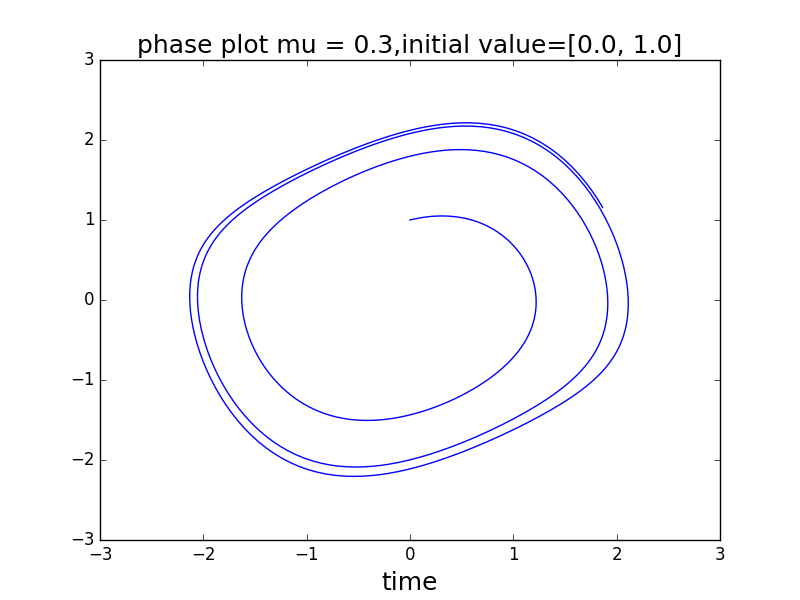
\includegraphics[width=8cm]{../output/phase_plot.png}
\end{center}
\caption{Phase plot}\label{lines}
\end{figure}

$$\frac{dx^n}{dx}=(n+1)x^{n}\text{ if }x\ne-1$$

A plot of position and velocity Vs time is shown in Figure 2.

\begin{figure}[!htbp]
\begin{center}
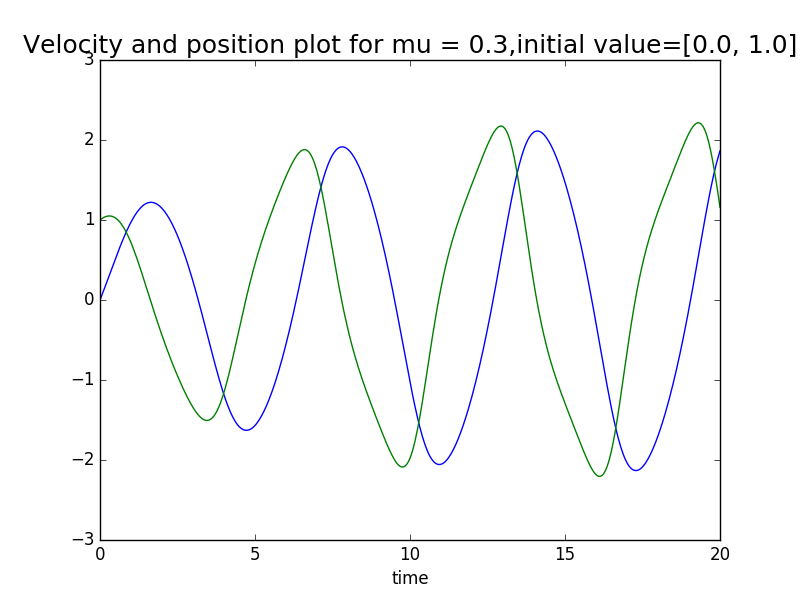
\includegraphics[width=8cm]{../output/position_velocity.png}
\end{center}
\caption{Position and Velocity Variations}\label{pos}
\end{figure}

\bibliographystyle{plain}
\bibliography{bibliography.bib}
\end{document}